% VUT FIT 2BIT
% IDS 2017/2018
% Semester project
% Author: Vladimir Dusek, xdusek27
% Date: 2/5/2018
% File: ids-doc.tex

%%%%%%%%%%%%%%%%%%%%%%%%%%%%%%%%%%%%%%%%%%%%%%%%%%%%%%%%%%%%%%%%%%%%%

\documentclass[12pt, a4paper, titlepage]{article}
\usepackage[left=2cm, text={17cm, 24cm}, top=3cm]{geometry}
\usepackage[utf8]{inputenc}
\usepackage[czech]{babel}
\usepackage{pdfpages}
\usepackage[obeyspaces]{url}
\usepackage{framed}
\usepackage[T1]{fontenc}
\usepackage{lmodern}

\setlength\parindent{0pt}

%%%%%%%%%%%%%%%%%%%%%%%%%%%%%%%%%%%%%%%%%%%%%%%%%%%%%%%%%%%%%%%%%%%%%

\begin{document}

\begin{titlepage}
	\begin{center}
		% {\Huge\textsc{Vysoké učení technické v~Brně}} \\
		% \bigskip
		% {\huge\textsc{Fakulta informačních technologií}} \\

		\begin{figure}[htb]
			\centering
			
\includegraphics[width=0.85\hsize]{fitlogo.pdf}
		\end{figure}

		\vspace{\stretch{0.382}}

		{\huge Databázové systémy} \\
		\medskip

		{\huge 2017/2018} \\
		\bigskip

		{\Huge \textbf{Dokumentace k~projektu}} \\
		\bigskip

		\vspace{\stretch{0.618}}
	\end{center}

	\begin{large}
		\hfill Vladimír Dušek (xdusek27)
		\medskip \\
		\today \hfill Tomáš Kukaň (xkukan00)
	\end{large}

\end{titlepage}

%%%%%%%%%%%%%%%%%%%%%%%%%%%%%%%%%%%%%%%%%%%%%%%%%%%%%%%%%%%%%%%%%%%%%

\tableofcontents
\newpage

%%%%%%%%%%%%%%%%%%%%%%%%%%%%%%%%%%%%%%%%%%%%%%%%%%%%%%%%%%%%%%%%%%%%%

\section{Zadání}
\medskip

Navrhněte fragment informačního systému pro prodej lístků na vlakové spoje. Systém bude umět odpovědět na dotazy typu jakou trasou zvolený spoj jede, jaké jsou vzdálenosti (časové) mezi zastávkami, jaký typ vlaku jede, průměrné zpoždění vlaku, apod. Doba přepravy mezi dvěma zastávkami může být různá v~závislosti na typu vlaku. Uvažujte více společností provozujících vlakové spoje. Různé vlaky nabízí různé služby (jídelní vůz, spací vůz, přeprava kol, apod.), za jejich využití se platí pevně daný příplatek. Dostupnost služby či velikost příplatku se liší v~závislosti na vlaku. Na základě uložených dat by si měl uživatel být schopen vyhledat spoj mezi dvěma zastávkami, zjistit dostupné služby a zjistit výslednou cenu přepravy. Uživatel si může přes internet koupit (a zrušit již zakoupenou) jízdenku a procházet historii svých jízdenek.
\bigskip

{\textit{Zadání je převzato z~předmětu IUS -- Lístky na vlak}

\clearpage

%%%%%%%%%%%%%%%%%%%%%%%%%%%%%%%%%%%%%%%%%%%%%%%%%%%%%%%%%%%%%%%%%%%%%

\section{Use case diagram}
\bigskip \bigskip \bigskip

\begin{figure}[htb]
	\centering
	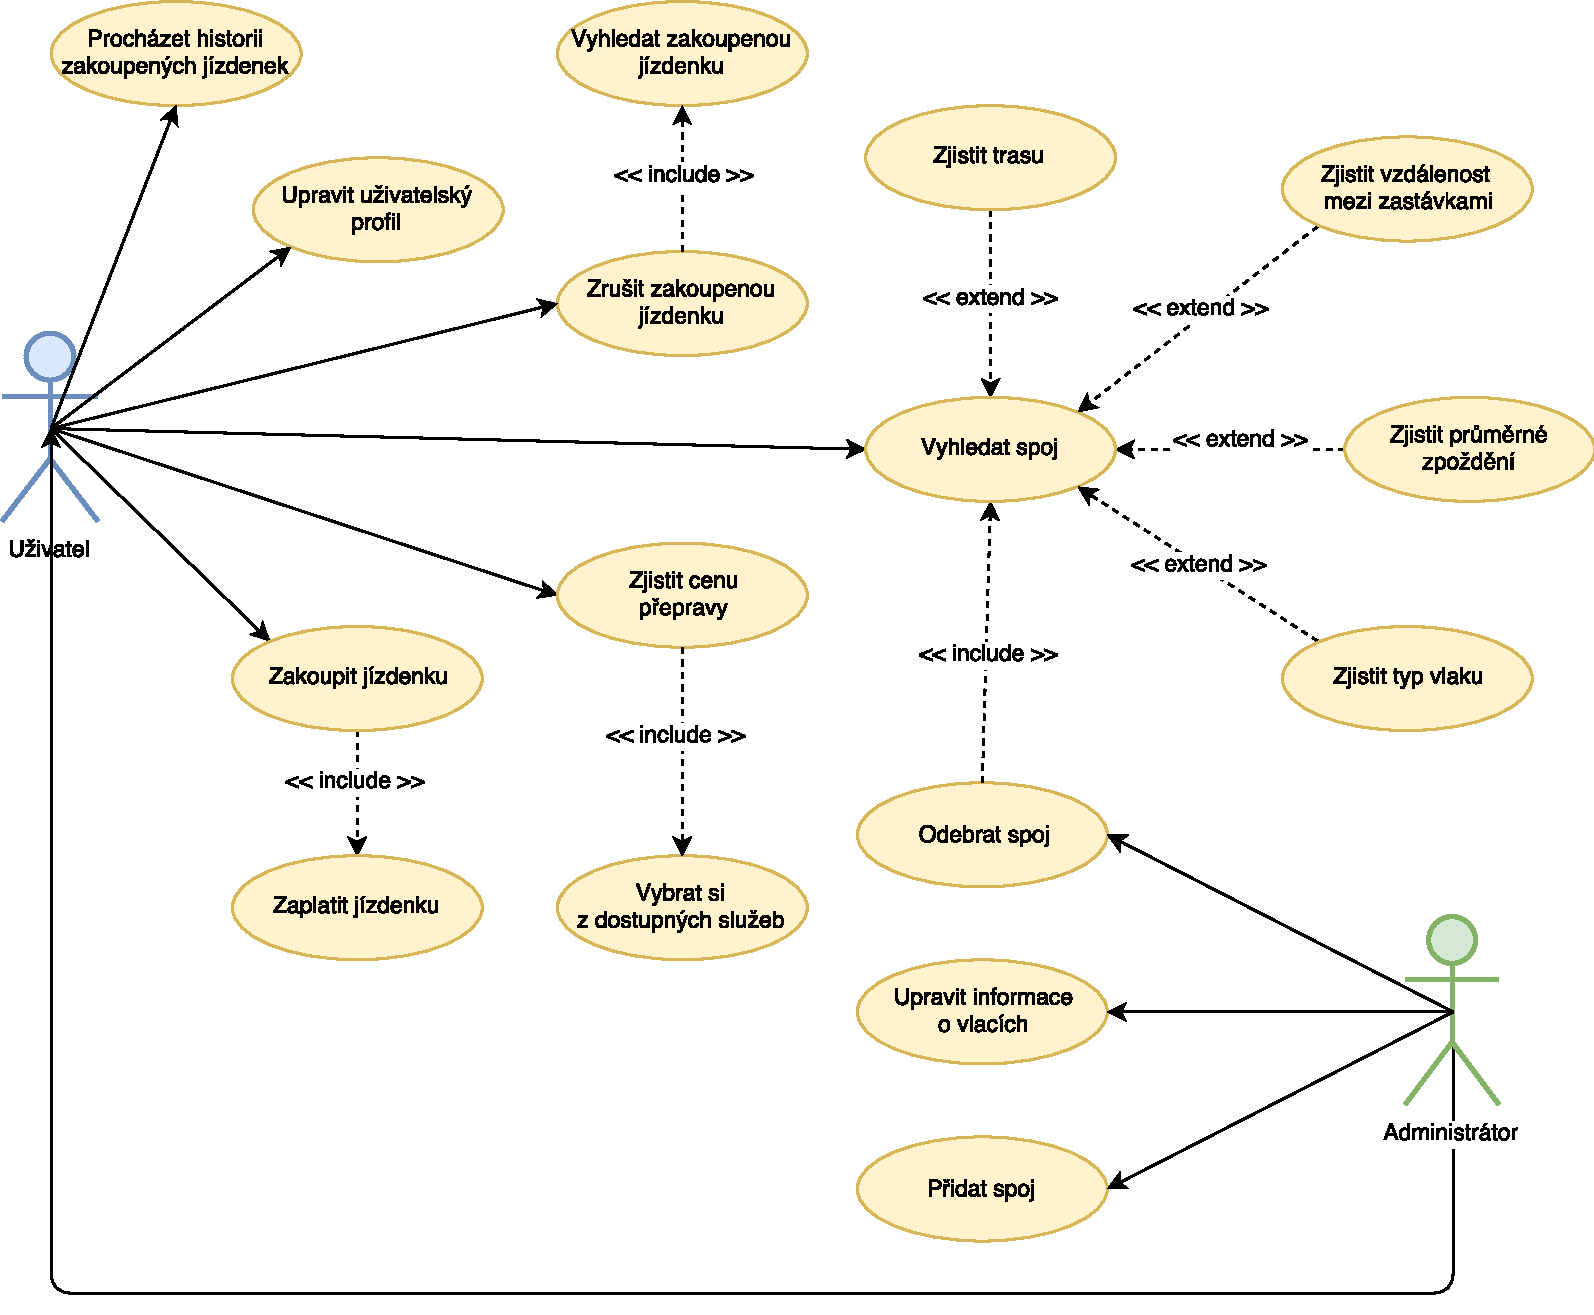
\includegraphics[width=0.8\hsize]{use_case.pdf}
\end{figure}

\clearpage

%%%%%%%%%%%%%%%%%%%%%%%%%%%%%%%%%%%%%%%%%%%%%%%%%%%%%%%%%%%%%%%%%%%%%

\section{Entity-relationship diagram}
\bigskip \bigskip \bigskip

\begin{figure}[htb]
	\centering
	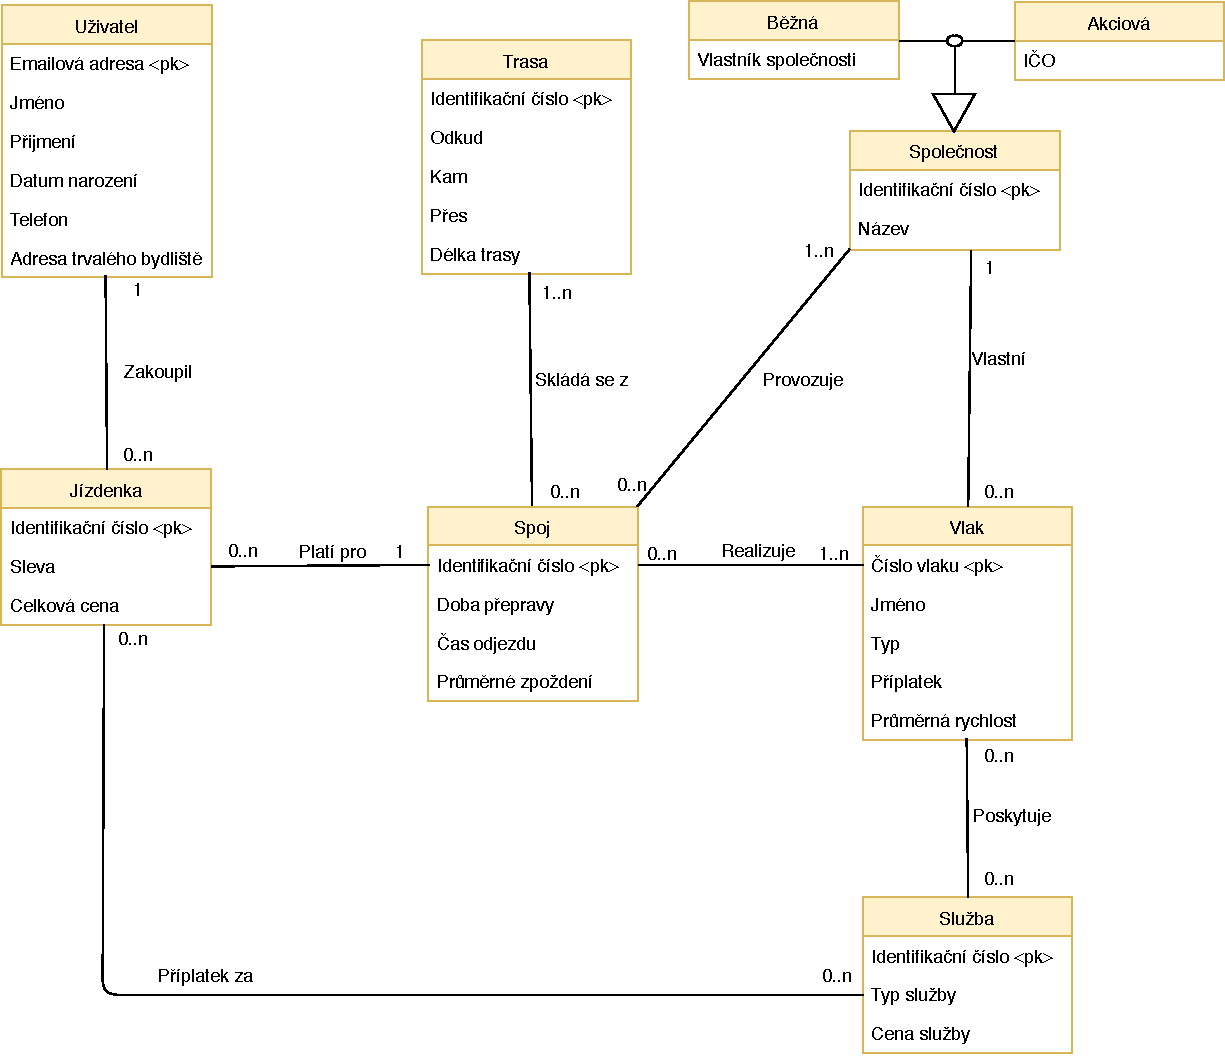
\includegraphics[width=0.8\hsize]{erd.pdf}
\end{figure}

\clearpage

%%%%%%%%%%%%%%%%%%%%%%%%%%%%%%%%%%%%%%%%%%%%%%%%%%%%%%%%%%%%%%%%%%%%%

\section{SQL skript}

Skript nejprve odstraní všechny databázové objekty kvůli zabránění potenciálním konfliktům. Postupně se vytvoří všechny tabulky a nastaví se jejich primární a cizí klíče. Tabulky jsou naplněny daty pro další práci s databází. Poté je vytvořeno několik triggerů a uložených procedur včetně otestování jejich funkcionality. Následuje několik dotazů select. Skript dále demonstruje využití indexu pro optimalizaci zpracování dotazu pomocí explain plan, dále využití materializovaného pohledu a přidělení přístupových práv k databázovým objektům druhému členovi týmu.
\medskip

%%%%%%%%%%%%%%%%%%%%%%%%%%%%%%%%%%%%%%%%%%%%%%%%%%%%%%%%%%%%%%%%%%%%%

\section{Triggery}

Implementovali jsme dva triggery. První přesně vyplývá ze zadání a slouží pro automatické generování hodnot primárního klíče, v našem případě je to id jízdenky -- \path{jizdenka_id_auto_inc}. Trigger se realizoval pomocí sekvence \path{sq_last_jizdenka_id}, která uchovává poslední vložené ID. Začíná se od 1 a postupně se inkrementuje.
\bigskip

Druhý trigger má identifikátor \path{check_spolecnost_ico} a slouží pro kontrolu správného zadání IČO společnosti. Trigger kontroluje jestli má IČO správnou délku (8 znaků), jestli se skládá pouze z číslic a také jestli je platné. Neprojde-li IČO kontrolou je vyvoláno chybové hlášení s kódem -20010 pomocí \path{raise_application_error}.
\medskip

%%%%%%%%%%%%%%%%%%%%%%%%%%%%%%%%%%%%%%%%%%%%%%%%%%%%%%%%%%%%%%%%%%%%%

\section{Uložené procedury}

Implementovali jsme také dvě uložené procedury. První \path{sp_kontrola_email} používá kurzor -- \path{cr_uzivatel} a proměnnou odkazující se na sloupec tabulky -- \path{ptr_column_email}. Slouží pro kontrolu správného formátu emailu uživatele. Neodpovídá-li formát, je vyhozena výjimka \path{ex_invalid_email}. Ta je později odchycena a je vyvoláno chybové hlášení s kódem -20020 pomocí \path{raise_application_error}.
\bigskip

Druhá procedura \path{sp_kontrola_vlak_id} funguje na podobném principu a slouží pro kontrolu id vlaku, tedy jestli se nejedná o záporné číslo. Nesplňuje-li id tuto podmínku je vyhozena výjimka \path{ex_invalid_id}. Ta je později odchycena a je vyvoláno chybové hlášení s kódem -20030 pomocí \path{raise_application_error}.

\clearpage

%%%%%%%%%%%%%%%%%%%%%%%%%%%%%%%%%%%%%%%%%%%%%%%%%%%%%%%%%%%%%%%%%%%%%

\section{Explain plan a vytvoření indexu}

\path{EXPLAIN PLAN} nám ukazuje jak je daný dotaz zpracováván databázovým strojem, dává nám tedy podněty k optimalizaci. Pro demonstraci možné optimalizace jsme vybrali dotaz, který spojí dvě tabulky, využije agregační funkci, klauzuli \path{GROUP BY} a vypíše jméno a přijmení uživatele a kolik celkem utratil v našem systému za jízdenky.
\bigskip

\path{EXPLAIN PLAN} pro náš dotaz vypadá následovně:

\begin{center}
\begin{figure}[h]
    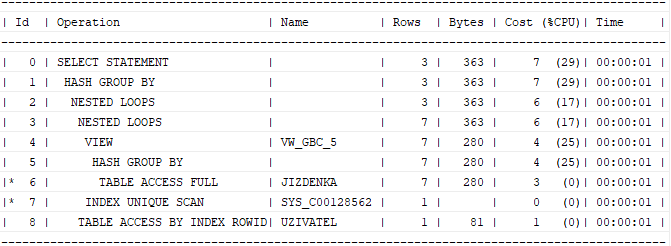
\includegraphics[scale=0.8]{ep_pred.png}
\end{figure}
\end{center}

Ve sloupci {\textit{Operation} můžeme vidět jaké operace by datábázový stroj vykonal pro provedení našeho dotazu. \path{SELECT STATEMENT} znamená, že se vykonal dotaz \path{SELECT}. \path{HASH GROUP BY} značí seskupení položek podle hashovacího klíče. \path{NESTED LOOPS} je vnořený cyklus. Následuje \path{TABLE ACCES FULL}, to nám značí přechod celou tabulkou bez použití indexů. \path{INDEX UNIQUE SCAN} značí jeden z přístupů k tabulkám přes B-strom. Ve sloupci {\textit{Cost} můžeme vidět cenu operace.
\bigskip

Pro optimalizaci našeho dotazu jsme vytvořili index pomocí příkazu \path{CREATE INDEX idx_uz_email ON Jizdenka(uzivatel_email)}, pro snažší přístup k emailu uživatele v tabulce \path{Jizdenka}. Znovu jsme spustili \path{EXPLAIN PLAN}.

\begin{center}
\begin{figure}[h]
    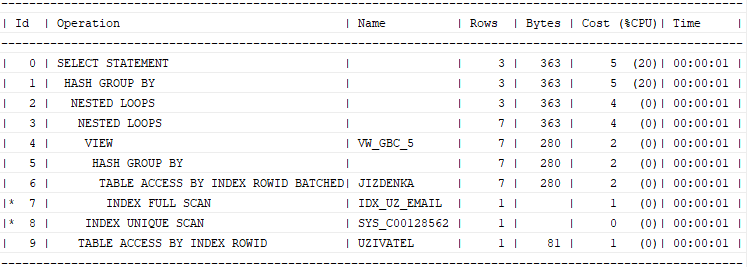
\includegraphics[scale=0.8]{ep_po.png}
\end{figure}
\end{center}

Jak můžeme vidět cena operací se snížila. Operace \path{TABLE ACCES BY INDEX ROWID BATCHED} nám říká, že do tabulky se přistupuje přes konkrétní řádek, databázový stroj tedy použil náš index.
\medskip

%%%%%%%%%%%%%%%%%%%%%%%%%%%%%%%%%%%%%%%%%%%%%%%%%%%%%%%%%%%%%%%%%%%%%

\section{Materializovaný pohled}

Nejprve jsme vytvořili materializované logy, kde se uchovávají změny původních tabulek. Ty jsou potřeba, abychom materializovanému pohledu mohli přiřadit vlastnost \path{FAST REFRESH ON COMMIT} místo výchozího \path{COMPLETE REFRESH}. Při tom se musí znovu spouštět celý dotaz materializovaného pohledu, což znamená vyšší cenu.
\bigskip

Poté jsme již vytvořili materializovaný pohled a demonstrovali jeho funkčnost na příkladu. Změnili jsme obsah původní tabulky, změny v materializovaném pohledu se projevili až po příkazu \path{COMMIT}. Materializovanému pohledu jsme dále nastavili vlastnosti \path{CACHE} -- optimalizace čtení z pohledu a \path{BUILD IMMEDIATE} -- naplnění pohledu ihned po jeho vytvoření.
\bigskip

Dále jsme pomocí příkazu \path{EXPLAIN PLAN} požádali o vysvětlení zpracování původního dotazu \path{SELECT}. Získali jsme přehled o jednotlivých operacích, které databázový stroj musí vykonat a jejich náročnosti.

\begin{center}
\begin{figure}[h]
    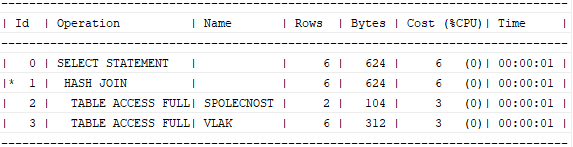
\includegraphics[scale=0.8]{mv_pred.png}
\end{figure}
\end{center}

Následně jsme požádali o vysvětlení zpracování dotazu \path{SELECT} našeho materializovaného pohledu.

\begin{center}
\begin{figure}[h]
    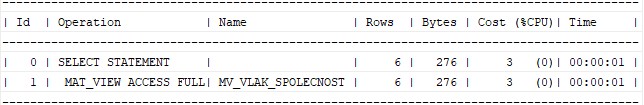
\includegraphics[scale=0.8]{mv_po.png}
\end{figure}
\end{center}

Dosáhli jsme snížení ceny, tedy menší zátěže CPU díky materializovanému pohledu.
\medskip

%%%%%%%%%%%%%%%%%%%%%%%%%%%%%%%%%%%%%%%%%%%%%%%%%%%%%%%%%%%%%%%%%%%%%

\section{Přídělení přistupových práv}

Druhý člen týmu má přidělená přístupová práva pomocí příkazu \path{GRANT}. Konkrétně \\ \path{GRANT ALL ON table_name TO login2} pro tabulky a materializovaný pohled a \\ \path{GRANT EXECUTE ON stored_procedure_name TO login2} pro uložené procedury. Druhý člen týmu se poté připojí k databázi prvního člena týmu pomocí příkazu \\ \path{ALTER SESSION SET CURRENT_SCHEMA = login1} a následně může s databázovými objekty pracovat.

%%%%%%%%%%%%%%%%%%%%%%%%%%%%%%%%%%%%%%%%%%%%%%%%%%%%%%%%%%%%%%%%%%%%%

\end{document}
